\documentclass[letterpaper]{article}

\usepackage[preprint]{aaai2027}

\usepackage[hyphens]{url}

\usepackage{graphicx}

\usepackage{natbib}

\usepackage{caption}

\usepackage{booktabs}

\usepackage{amsmath}

\frenchspacing

\urlstyle{rm}

\def\UrlFont{\rm}

\setcounter{secnumdepth}{0}

\title{Reference-Aware Gait Anomaly Detection for Medical World Models}

\author{Author details pending confirmation}

\affiliations{Affiliation pending confirmation}

\begin{document}

\maketitle

\begin{abstract}

Gait video can describe how a person's movement changes, but prediction error needs a reference before it can serve as an anomaly score. A restricted yet repeatable gait can be easier to predict than ordinary walking. We present a source-grouped benchmark that compares learned forecasts with persistence, which repeats the last observed pose. Normal-only models predict eight future samples from public gait videos. Across 2,815 windows from 91 source videos, the bilateral model reduces normal-source forecast error by 33.5\%. Its prespecified excess error above persistence ranks abnormal annotations with AUROC 0.793, compared with 0.304 for raw forecast error. A post hoc low-movement diagnostic reaches 0.806, showing why the reference itself must be evaluated. Current posture also forecasts better than bilateral history. These results provide a practical way to separate forecasting skill, movement amount, and anomaly ranking. They support an exploratory motor-observation benchmark, without establishing clinical diagnosis or a learned anomaly advantage over movement alone.

\end{abstract}

\section{Introduction}

A medical world model needs observations that describe a patient's state and a model of how that state changes. Gait provides one possible observation. Videos reveal relative motion of the legs even when clinical sensors are unavailable. Before these observations support clinical simulation, however, we need to know what their prediction errors mean.

A common approach trains on normal movement and treats large prediction errors as evidence of abnormality. This assumes that abnormal movement is harder to predict. The assumption can fail when a restricted or repeatable pattern produces little change between frames. Repeating the last pose can then obtain a small error without describing healthy movement.

We address this problem with a reference-aware evaluation. The same observed future is scored against a learned forecast and against persistence. Their difference describes how much the learned model helps beyond holding the last pose fixed. We then evaluate the reference itself, the importance of movement history, and the effect of keeping source videos separate. The contribution is a reproducible benchmark and an interpretable score analysis. It provides a practical test of whether a gait observation model learns information useful for anomaly ranking beyond simple movement differences.

\begin{figure*}[t]

\centering

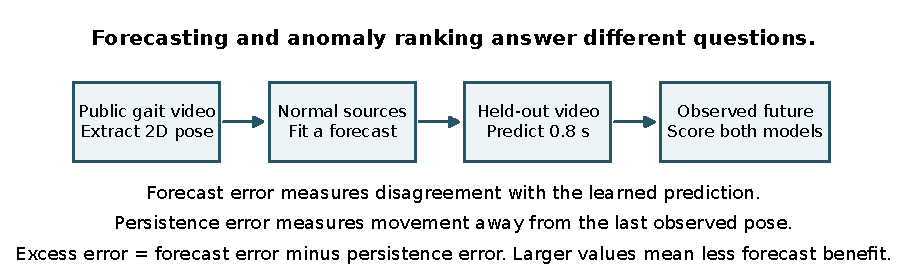
\includegraphics[width=\textwidth]{figures/method.pdf}

\caption{The workflow separates model fitting from held-out scoring. Both forecasts are compared with exactly the same observed future. The anomaly score becomes available only after that future is observed.}

\end{figure*}

\section{Neurological motivation and related work}

Walking coordinates body segments while maintaining support and advancing the body. Laboratory measurements show structured relationships between segment angles \citep{borghese1996}. Bilateral timing is clinically relevant: Plotnik and colleagues measured changes in the coordination of left and right steps in Parkinson's disease \citep{plotnik2007}. Studies of stroke and cerebral palsy link altered muscle-activation patterns with impaired walking \citep{clark2010,steele2015}. These observations motivate testing relationships between the legs. They do not imply that every disorder increases prediction error or that video coordinates identify a neural mechanism. The myopathic annotation also describes a neuromuscular category, rather than a shared neurological cause across all included conditions.

MoCoDAD uses skeleton forecasts for anomaly detection \citep{flaborea2023}. FSGait combines normal-only gait reconstruction and prediction to detect postural and temporal abnormalities \citep{duan2024}. GenGait studies normative reconstruction \citep{motta2026}, while S-JEPA predicts hidden skeleton representations for action recognition \citep{abdelfattah2024}. Normal-only gait prediction is therefore established prior art. Following the importance of simple motion references \citep{martinez2017}, our contribution evaluates forecast skill and anomaly scores under one timing, observation, and source-grouping contract.

\section{Data and observation contract}

The pinned local GAVD inventory contains 1,874 sequences from 348 source IDs \citep{ranjan2025}. The five selected annotations contain 666 sequences from 103 sources. Available-media checks retain 652 sequences from 98 sources. Two documented source exclusions for identity or scene problems leave 641 extraction candidates from 96 sources. Timing, geometry, observation, and common-target gates retain 2,815 windows from 456 sequences and 91 sources. These video groups are not verified independent participants.

Ambient performs 46,783 recorded pose-model calls over the available annotated spans. We sample nearest native frames on a nominal 10 Hz grid and retain actual frame numbers and times. Each window has 16 observed and eight future samples, with stride eight. The observed prefix spans 1.5 seconds. The final future sample occurs 0.767 to 0.834 seconds later. We evaluate all eight future samples, not only the final instant.

The contract uses 16 BlazePose joints, confidence at least 0.5, and at least 70\% valid observations separately in the prefix and future. An annotation-box check rejects unresolved geometry, although it cannot guarantee identity in crowded scenes. Coordinates are centered on each frame's pelvis and divided by a prefix-only torso scale. They describe relative 2D articulation, not physical speed. Both hips define the reference, so the own-leg model does not have strictly unilateral visual access.

Observation gates retain different fractions of the annotations. For example, 141 of 287 normal extraction candidates remain, compared with 168 of 183 myopathic candidates. All 32 annotated normal source IDs are already in the selected scope. Other GAVD labels cannot increase this normal-source ceiling, and additional windows do not create independent people.

\begin{table}[t]
\centering
\small
\begin{tabular}{lrrr}
\toprule
Annotation & Sources & Sequences & Windows \\
\midrule
Cerebral palsy & 8 & 52 & 518 \\
Myopathic & 27 & 168 & 845 \\
Normal & 29 & 141 & 465 \\
Parkinsons & 11 & 37 & 292 \\
Stroke & 16 & 58 & 695 \\
\bottomrule
\end{tabular}
\caption{The evaluated cohort groups observations by source video. Counts do not establish independent participants.}
\end{table}

\section{Forecasts and anomaly scores}

For each target leg, ridge regression predicts future knee, ankle, heel, and foot-index coordinates. This linear model penalizes large coefficients to limit overfitting. Inputs use eight fixed prefix positions, including both endpoints, with observation indicators. Missing values are filled from earlier prefix observations only. Outputs are trained only where future targets were observed.

The own-leg model uses that leg's history. The bilateral model adds the opposite leg. A separately trained timing control shifts the seven earlier opposite-leg samples by a window-specific offset while preserving their values, validity, and current anchor. The current-posture model learns a separate transition at each future time from the latest bilateral pose. Its output can change over time. Persistence instead holds the latest pose fixed. Damped velocity and declared shrinkage variants provide additional references.

Let $a$ be the latest observed coordinate, $y$ its observed future, and $\widehat y$ the learned prediction. Actual displacement is $d = y - a$ and predicted displacement is $u = \widehat y - a$. Excess squared error is $(d - u)^2 - d^2 = u^2 - 2du$. The identity also holds after averaging with the same observed-coordinate support and hierarchical weights. Excess error therefore combines prediction size and alignment with actual movement. Subtracting persistence does not remove every effect of movement amount, view, or pose noise.

Larger excess error is prespecified to indicate more abnormal gait. A negative value means forecasting improved on persistence. Other declared scores are raw bilateral error, persistence error, bilateral-minus-own error, and prefix missingness. Because all error scores require the observed future, they detect anomalies retrospectively within a sequence. They do not predict an abnormal event before it occurs.

\section{Evaluation}

Five outer folds keep all sequences and windows from one source together. Models train only on normal sources outside the evaluation fold. Three inner source folds select regularization from 0.1, 1, 10, and 100. Scaling is refitted within every training split. A secondary analysis blends learned displacement with persistence using strengths 0, 0.25, 0.5, or 1, selected on inner normal-source validation. Abnormal labels do not select model settings.

All methods share observed future targets. We average coordinate errors within a leg and window, the two legs equally, then windows within sequences, sequences within sources, and sources equally. Training weights follow this hierarchy. Forecast evaluation uses 29 normal sources. Anomaly ranking compares 62 abnormal and 29 normal sources. AUROC is the probability that an abnormal source receives a higher score than a normal source; average precision also depends on prevalence.

The frozen analysis uses 5,000 source resamples for forecast intervals and 2,000 stratified source resamples for anomaly intervals. These intervals condition on fixed models with overlapping training folds. They exclude retraining and participant-population uncertainty. The study is exploratory because GAVD outcomes were available during research development.

This report adds an explicitly post hoc low-movement diagnostic: negative persistence error. It assigns larger scores to smaller observed movements without changing any frozen score direction. We compare it with excess error using 5,000 paired stratified source resamples. Within-fold rankings avoid comparing scores from different fitted models. These added analyses do not select a model, threshold, or clinical rule.

\section{Results}

Normal-source mean squared error is 0.12126 for persistence and 0.08063 for bilateral forecasting. The paired reduction is 0.04063 [0.02399, 0.05911], or 33.5\% of the persistence mean. Bilateral forecasting improves error on 23 of 29 normal sources. This establishes useful forecast information within the observation contract.

The gain over own-leg history is 0.00111 [-0.00253, 0.00524], and the gain over the trained timing control is 0.00591 [0.00141, 0.01134]. However, current posture forecasts better, with error 0.07164, a 40.9\% reduction from persistence. Longer bilateral context is therefore not established as necessary. Shrinkage yields bilateral error 0.08378 and does not improve the unshrunk model.

Prespecified excess error achieves AUROC 0.793 [0.680, 0.896] and average precision 0.865 [0.788, 0.938]. Raw forecast error has AUROC 0.304 [0.178, 0.431], and persistence error has AUROC 0.194 [0.096, 0.300]. Abnormal-source prevalence is 0.681. These differences show that an error-based ranking depends strongly on its reference and interpretation.

The post hoc low-movement diagnostic has AUROC 0.806. The paired difference, excess error minus low movement, is -0.013 [-0.111, 0.083]. This does not establish added anomaly-ranking value from the learned forecast. Excess-error AUROC within individual folds ranges from 0.653 to 0.931. Weighting those rankings by the number of normal-abnormal source pairs gives 0.774, compared with 0.811 for low movement. Their paired difference is -0.036 [-0.145, 0.067]. The association persists without cross-fold pairs, while small source groups produce substantial variation. Complete scores and condition slices appear in the appendix.

\begin{figure}[t]

\centering

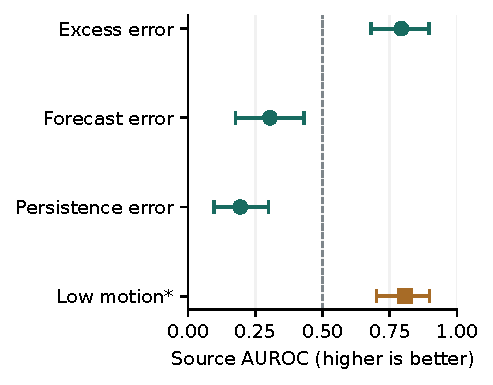
\includegraphics[width=\columnwidth]{figures/anomaly_scores.pdf}

\caption{Ranking across 91 source videos (29 normal and 62 abnormal) depends on the reference. Bars show conditional 95\% source intervals. The asterisk marks a post hoc diagnostic that assigns higher scores to less movement. It is not a validated clinical score.}

\end{figure}

\section{Discussion and limitations}

The study supplies a useful observation-model benchmark and a concrete lesson for gait anomaly detection. A model can forecast normal movement well while its raw error ranks restricted abnormal movement as easier. Comparing forecasts with persistence exposes this distinction. Evaluating persistence as an anomaly diagnostic then tests whether the apparent benefit comes from learned behavior or movement amount. This sequence of checks is the methodological contribution.

The next model should demonstrate added information beyond current posture and movement-only scores. Promising tests include normal-only calibration conditional on prefix motion and view, and structured masks that hide a leg or a continuous time interval. Such masks could encourage use of coordination rather than nearby redundant samples. These are proposed extensions that require matched budgets, fixed targets, timing controls, and an untouched evaluation cohort.

GAVD supports exploratory evaluation across heterogeneous public-video sources, but does not establish clinical generalizability. Participants may recur across uploads, a video may contain several people, and local annotations do not independently verify diagnoses. View, age, walking task, assistive devices, acquisition quality, and unequal retention can influence scores. More overlapping windows cannot resolve these limitations or enlarge the 29 retained normal-source groups.

The model describes short-term articulation without treatment inputs, repeated clinical visits, or measured intervention outcomes. Patient-level decisions require external participant-disjoint data and validated clinical measurements. Within this scope, the benchmark separates forecasting skill from anomaly ranking and defines clear tests for stronger medical claims.

\clearpage

\bibliography{references}

\clearpage

\appendix

\section{Complete exploratory results}

All original forecast arms and prespecified score directions are retained. Added diagnostics are explicitly post hoc.

\begin{center}

\begin{minipage}{\columnwidth}

\centering

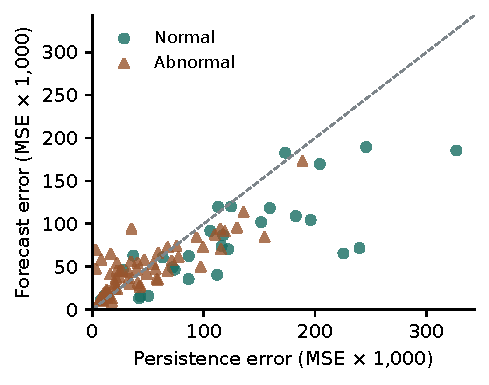
\includegraphics[width=\columnwidth]{figures/source_errors.pdf}

\captionof{figure}{The 91 source videos comprise 29 normal and 62 abnormal sources. Axes show squared body-relative coordinates, normalized by prefix torso scale and multiplied by 1,000. Points below the equal-error line benefit from forecasting. Normal sources often have larger errors on both axes, explaining the direction of raw-error ranking.}

\end{minipage}

\end{center}

\begin{center}\begin{minipage}{\columnwidth}
\centering
\small
\begin{tabular}{lrr}
\toprule
Score & AUROC [95\% interval] & AP \\
\midrule
Bilateral MSE & 0.304 [0.178, 0.431] & 0.558 \\
Persistence MSE & 0.194 [0.096, 0.300] & 0.519 \\
Excess MSE & 0.793 [0.680, 0.896] & 0.865 \\
Bilateral minus own & 0.549 [0.410, 0.684] & 0.694 \\
Prefix missingness & 0.427 [0.296, 0.555] & 0.646 \\
\bottomrule
\end{tabular}
\captionof{table}{All prespecified anomaly scores.}
\end{minipage}\end{center}

\begin{center}\begin{minipage}{\columnwidth}
\centering
\small
\begin{tabular}{lr}
\toprule
Forecast & MSE × 1,000 \\
\midrule
Persistence & 121.262 \\
Damped velocity & 267.828 \\
Own-leg history & 81.744 \\
Bilateral history & 80.632 \\
Shifted bilateral & 86.541 \\
Static posture & 71.636 \\
Shrunk bilateral & 83.779 \\
\bottomrule
\end{tabular}
\captionof{table}{Normal-source forecast error over all eight future samples.}
\end{minipage}\end{center}

\begin{center}\begin{minipage}{\columnwidth}
\centering
\small
\begin{tabular}{lr}
\toprule
Forecast & MSE [95\% interval] \\
\midrule
Bilateral history & 71.838 [54.566, 91.196] \\
Shrunk bilateral & 76.246 [58.289, 96.254] \\
Damped velocity & 157.107 [110.674, 210.279] \\
Inference shift & 86.547 [67.969, 108.831] \\
Inference static & 68.688 [52.774, 86.527] \\
Own-leg history & 71.231 [54.991, 89.393] \\
Shrunk own-leg & 73.086 [56.702, 91.336] \\
Persistence & 101.710 [74.483, 131.526] \\
Shifted bilateral & 75.449 [57.943, 95.573] \\
Shrunk shifted & 73.407 [55.687, 93.848] \\
Static posture & 64.166 [48.454, 81.562] \\
Shrunk static & 64.166 [48.454, 81.562] \\
\bottomrule
\end{tabular}
\captionof{table}{All forecasts through 0.4 seconds. MSE is multiplied by 1,000.}
\end{minipage}\end{center}

\begin{center}\begin{minipage}{\columnwidth}
\centering
\small
\begin{tabular}{lr}
\toprule
Reference / forecast & Gain [95\% interval] \\
\midrule
Persistence / Bilateral & 29.872 [12.220, 50.128] \\
Own / Bilateral & -0.607 [-4.023, 2.979] \\
Shifted / Bilateral & 3.611 [-0.260, 7.751] \\
Static / Bilateral & -7.672 [-13.888, -1.271] \\
Perturbed time / Bilateral & 14.709 [8.969, 20.812] \\
Perturbed static / Bilateral & -3.150 [-11.091, 5.259] \\
Persistence / Bilateral (S) & 25.464 [11.897, 40.421] \\
Bilateral / Bilateral (S) & -4.408 [-10.995, 0.616] \\
Own (S) / Bilateral (S) & -3.161 [-6.742, 0.224] \\
Shifted (S) / Bilateral (S) & -2.840 [-9.688, 3.336] \\
Static (S) / Bilateral (S) & -12.081 [-18.263, -6.063] \\
\bottomrule
\end{tabular}
\captionof{table}{Paired effects through 0.4 seconds. Positive values favor the forecast; values are multiplied by 1,000. S denotes shrinkage.}
\end{minipage}\end{center}

\begin{center}\begin{minipage}{\columnwidth}
\centering
\small
\begin{tabular}{lr}
\toprule
Forecast & MSE [95\% interval] \\
\midrule
Bilateral history & 80.632 [62.522, 100.023] \\
Shrunk bilateral & 83.779 [66.582, 102.528] \\
Damped velocity & 267.828 [193.236, 353.148] \\
Inference shift & 94.855 [75.079, 116.534] \\
Inference static & 82.261 [65.641, 100.124] \\
Own-leg history & 81.744 [64.066, 100.723] \\
Shrunk own-leg & 82.741 [66.126, 100.615] \\
Persistence & 121.262 [94.150, 150.800] \\
Shifted bilateral & 86.541 [67.032, 108.215] \\
Shrunk shifted & 84.278 [65.702, 104.376] \\
Static posture & 71.636 [55.850, 88.622] \\
Shrunk static & 71.636 [55.850, 88.622] \\
\bottomrule
\end{tabular}
\captionof{table}{All forecasts through 0.8 seconds. MSE is multiplied by 1,000.}
\end{minipage}\end{center}

\begin{center}\begin{minipage}{\columnwidth}
\centering
\small
\begin{tabular}{lr}
\toprule
Reference / forecast & Gain [95\% interval] \\
\midrule
Persistence / Bilateral & 40.630 [23.993, 59.111] \\
Own / Bilateral & 1.112 [-2.525, 5.244] \\
Shifted / Bilateral & 5.909 [1.407, 11.336] \\
Static / Bilateral & -8.996 [-15.894, -2.068] \\
Perturbed time / Bilateral & 14.224 [8.375, 20.592] \\
Perturbed static / Bilateral & 1.629 [-7.975, 11.520] \\
Persistence / Bilateral (S) & 37.483 [23.277, 53.257] \\
Bilateral / Bilateral (S) & -3.147 [-7.493, 0.494] \\
Own (S) / Bilateral (S) & -1.038 [-4.612, 3.182] \\
Shifted (S) / Bilateral (S) & 0.499 [-5.119, 6.375] \\
Static (S) / Bilateral (S) & -12.143 [-18.240, -6.523] \\
\bottomrule
\end{tabular}
\captionof{table}{Paired effects through 0.8 seconds. Positive values favor the forecast; values are multiplied by 1,000. S denotes shrinkage.}
\end{minipage}\end{center}

\begin{center}\begin{minipage}{\columnwidth}
\centering
\small
\begin{tabular}{lrrr}
\toprule
Fold & N/A & Excess & Low motion \\
\midrule
0 & 6/13 & 0.705 & 0.910 \\
1 & 6/12 & 0.931 & 0.931 \\
2 & 6/12 & 0.889 & 0.833 \\
3 & 6/12 & 0.653 & 0.778 \\
4 & 5/13 & 0.692 & 0.569 \\
\bottomrule
\end{tabular}
\captionof{table}{Post hoc within-fold AUROCs. N/A gives normal/abnormal source counts. Folds share training sources.}
\end{minipage}\end{center}

\begin{center}\begin{minipage}{\columnwidth}
\centering
\small
\begin{tabular}{lrrr}
\toprule
Annotation & Abnormal & Excess & Low motion \\
\midrule
Parkinsons & 11 & 0.856 & 0.868 \\
Stroke & 16 & 0.864 & 0.877 \\
Cerebral palsy & 8 & 0.690 & 0.759 \\
Myopathic & 27 & 0.756 & 0.754 \\
\bottomrule
\end{tabular}
\captionof{table}{Post hoc AUROC by annotation versus the same 29 normal sources. Small groups and repeated normal comparisons limit interpretation.}
\end{minipage}\end{center}

\section{Reproduction}

Targets are BlazePose joints 25, 27, 29, and 31 on the left, and 26, 28, 30, and 32 on the right. Each leg requires at least four observed joint-time points through four future samples and eight through all eight samples. Each target joint also requires at least one prefix observation. This common support gate removes three of the 2,818 prepared windows for every model. The completed run contains 80 saved fold, leg, and variant checkpoints, some sharing fitted coefficients. There are 29 normal source groups, not 80 independent replications. Evidence tables, hashes, notebook records, and source generators accompany this manuscript. Figures and diagnostics are regenerated from frozen artifacts; the manuscript builder never refits a model.

\end{document}
